%=======================+=========================
%================  Online  ================
%=================================================

%------------------------------------------------------------------
\section[Online computing system]{Online computing system \label{sec:online}}

This section describes the \GX ~software and computing systems  used for data monitoring and for transport to the tape system for permanent storage.

%------------------------------------------------------------------
\subsection{Monitoring \label{sec:onlinemonitoring}}

The Online Monitoring system consists of multiple stages that provide immediate monitoring of the data, as well as near-term monitoring (a few hours after acquisition). Immediate monitoring is based on the \textit{RootSpy} system\cite{rootspy} written for use in \GX, though its design is not experiment specific. Figure \ref{fig:online_monitoring_processes} shows a diagram of the processes involved in the RootSpy system and how those processes are coupled to the DAQ system. The Event Transfer System (ET) process is part of the CODA DAQ system \cite{coda} and is used to extract a copy of a portion of the datastream without interfering with data acquisition. The monitoring system uses a secondary ET to minimize connections to the RAID server running the Event Recorder process.

\begin{figure}[tbp]
\begin{center}
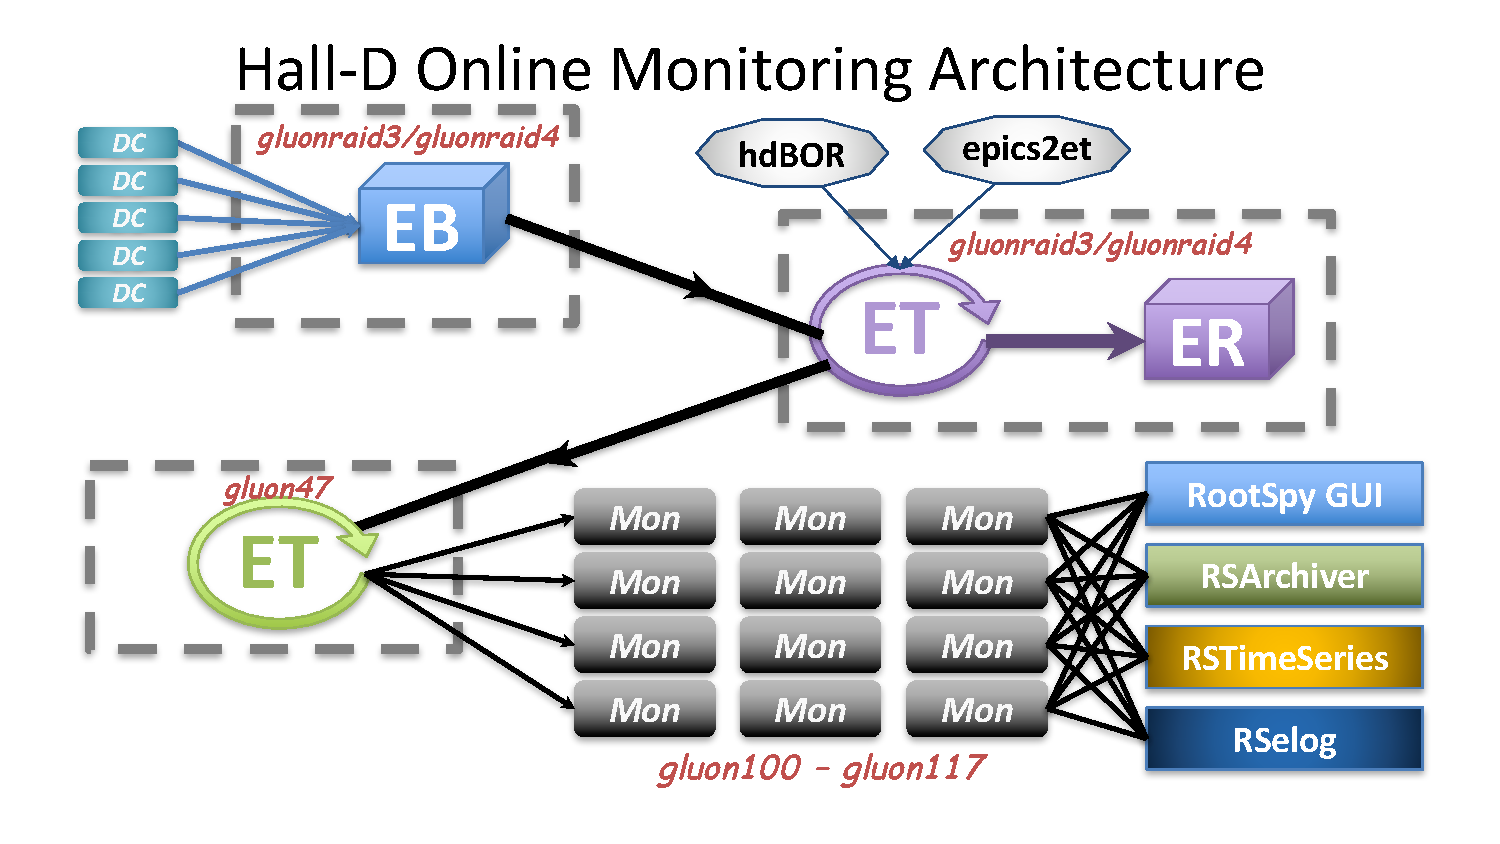
\includegraphics[width=0.99\textwidth, clip,trim=1.5cm 0.9cm 1.7cm 0.8cm]{figures/online_monitoring_processes.pdf}
\caption{\label{fig:online_monitoring_processes}Processes distributed across several computers in the online monitoring system. DC, EB, and ER are the Data Concentrator, Event Builder, and Event Recorder processes, respectively, in the CODA DAQ system.}   
\end{center}  
\end{figure}

The monitoring system is run on a small computer farm\footnote{The online monitoring farm consists of eight 2012 era Intel x86\_64 computers with 16 cores+16 hyper-threads (ht) plus six 2016 era Intel x86\_64 computers with 36 cores + 36ht. The monitoring farm uses 40 Gbps (QDR) and 56 Gbps(FDR) IB for the primary interconnect. Note that the DAQ system uses a separate 40 Gbps ethernet network that is independent of the farm.} in the counting house, each processing a small part of the data stream. In total, about 10\% of the data is processed for the low level occupancy plots while roughly 2\% is fully reconstructed for higher level analysis. The CODA ET software system is used to distribute the data among the farm computers. Each farm node generates histograms, which \textit{RootSpy} gathers and combines before display to shift workers in a GUI.
%Figure \ref{fig:online_monitoring_rootspy} shows a screen capture of the main RootSpy GUI window along with a window displaying the reference plot for the currently displayed image.
Plots are displayed via a set of ROOT macros, each responsible for drawing a single page. Most macros divide the page into multiple sections so that multiple plots can be displayed on a single page. Figure \ref{fig:online_monitoring_PID} shows an example of a high-level monitoring plot, where four invariant-mass distributions are shown with fits. Values extracted from the fits are printed on the plots for easy quantitative comparison to the reference plot. 

%Shift workers are presented with live plots alongside reference plots for comparison. Shift workers may assign a live plot as the new reference using a button on the \textit{RootSpy} GUI. Relevant experts for the given plot are notified via e-mail when a new reference is made, thus providing for expert oversight of the reference plots.

% ROOT macros are passed into the RootSpy GUI using the same xMsg\cite{xmsg} publish subscribe messaging system used to transport histogram objects. The macros are compiled into plugins as C++ strings by the build system. The build system recognizes ROOT macro files in the plugin source directory (via the .C suffix) and automatically generates C++ code that contains the macro and code to register it with the RootSpy system. This is done to ensure that a macro is always in sync with the histograms it displays since the former is linked in the same binary as the routines that produce the latter.

\begin{figure}[tbp]
\begin{center}
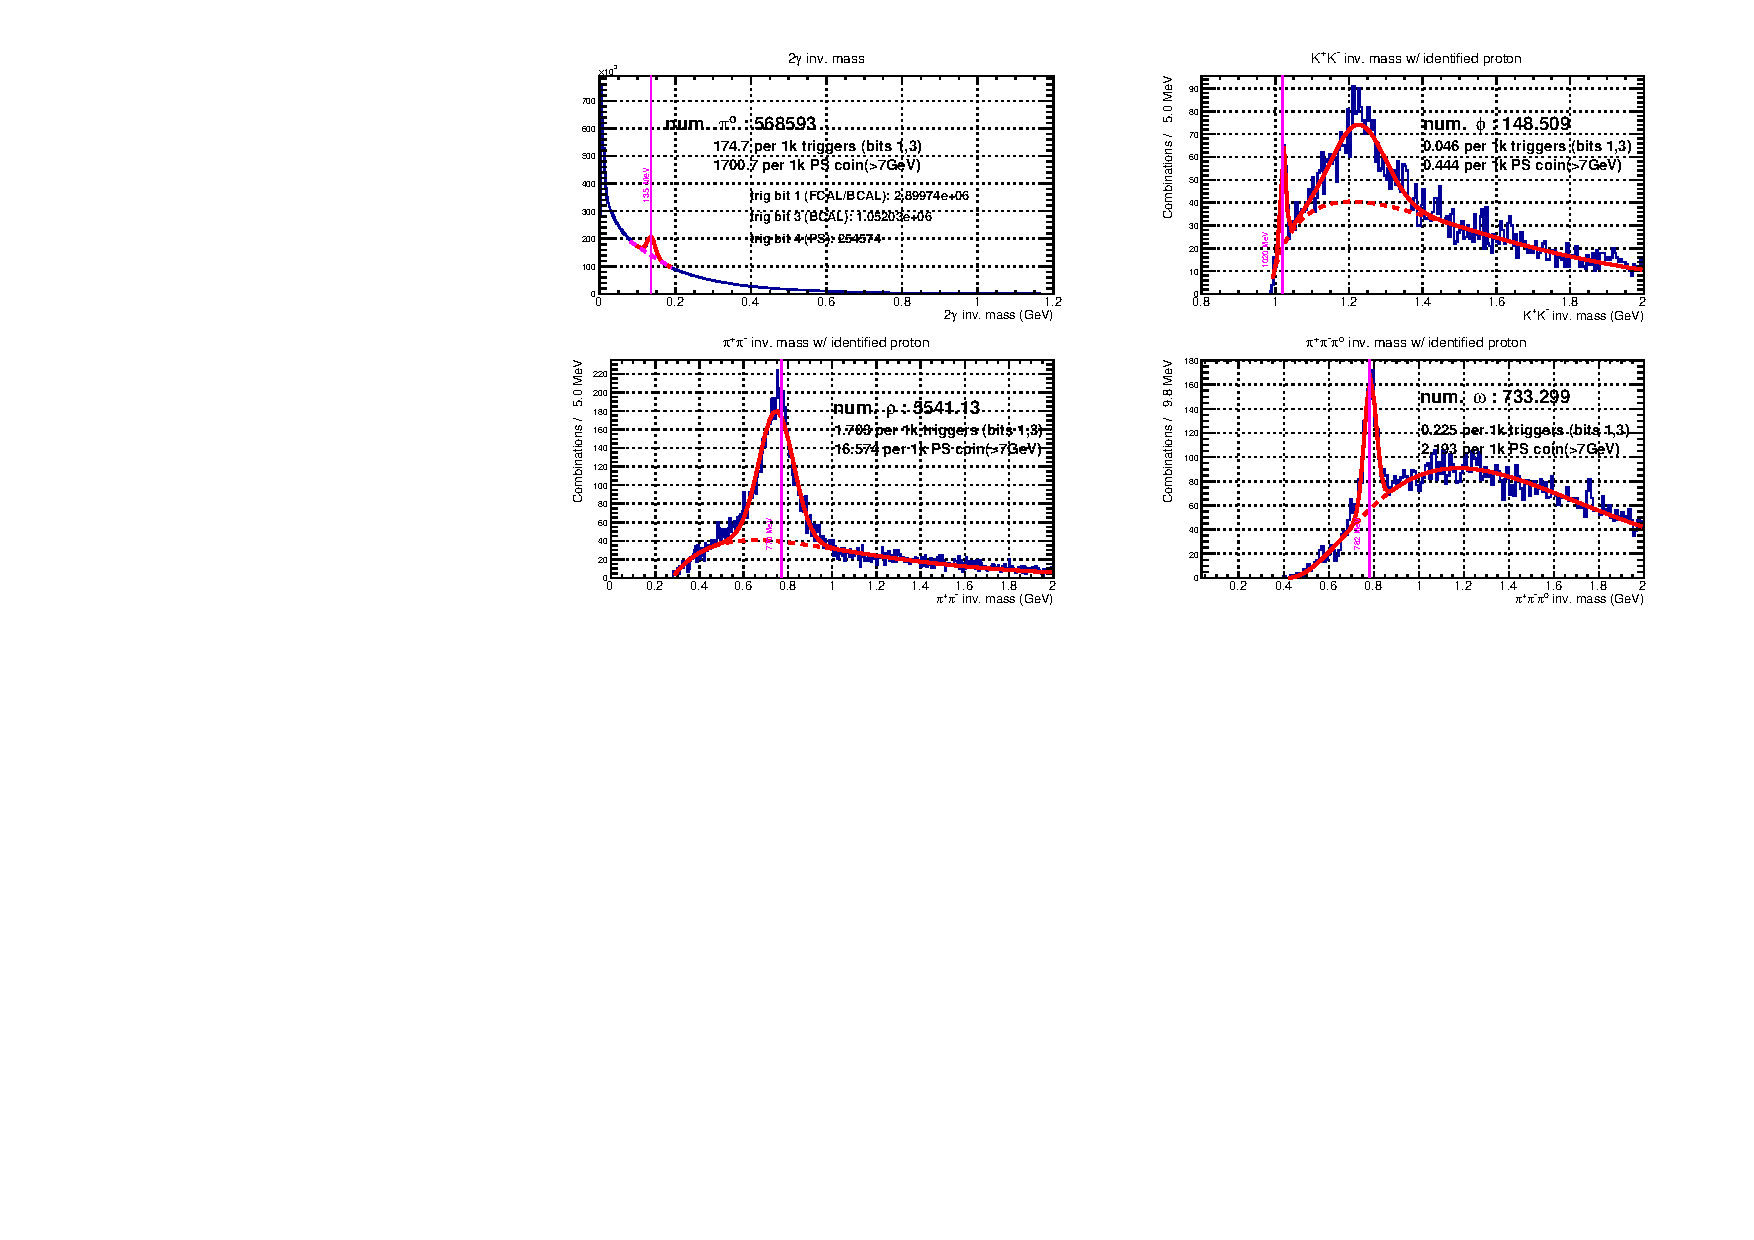
\includegraphics[width=0.99\textwidth]{figures/online_monitoring_PID.pdf}
%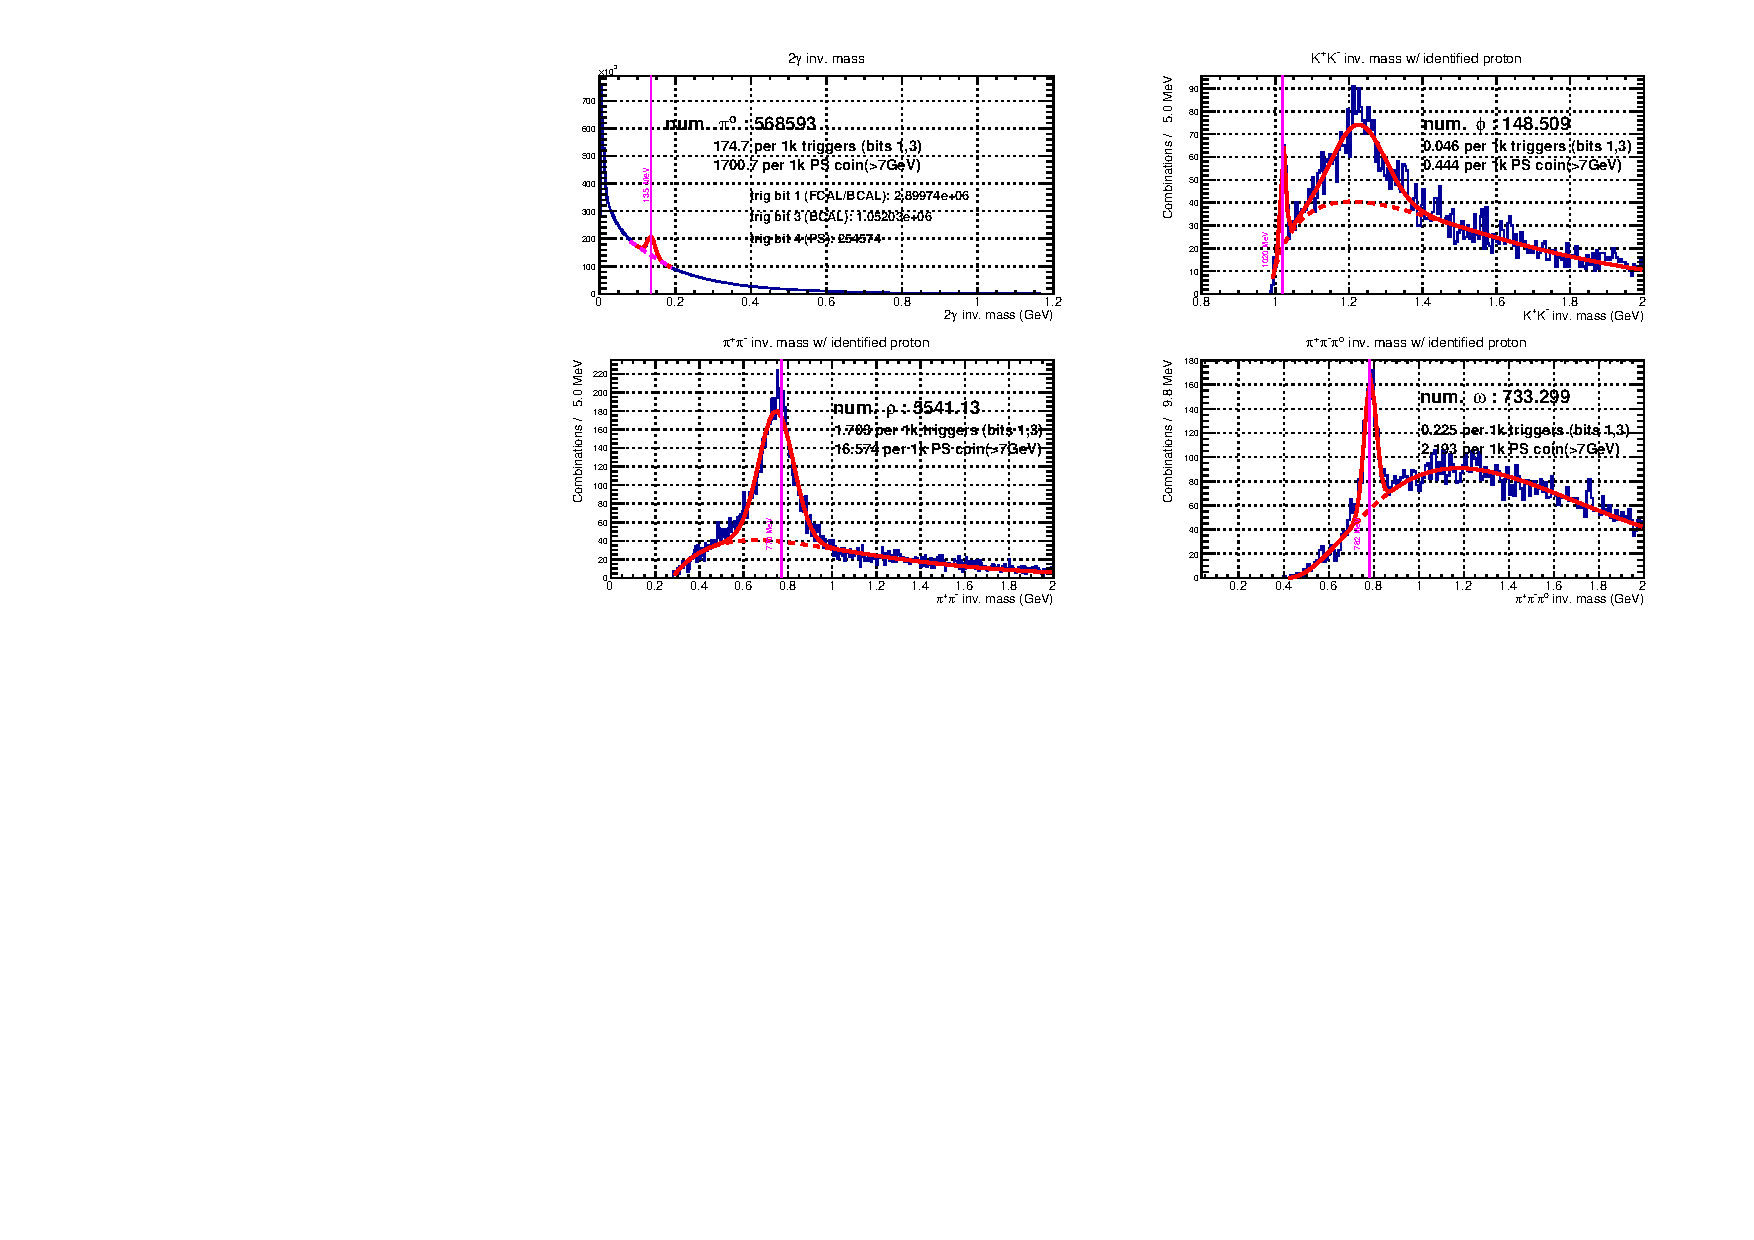
\includegraphics[width=0.99\textwidth, clip,trim=0.6cm 0.0cm 1.1cm 0.0cm]{figures/online_monitoring_PID.pdf}
\caption{\label{fig:online_monitoring_PID}Invariant mass distributions showing $\pi^\circ$, $\omega$, $\rho$, and $\phi$ particles. These plots were generated online in about 1hr 40min by looking at roughly 2\% of the data stream.}   
\end{center}  
\end{figure}

There are several client programs that summarize the information available in the histograms produced by \textit{RootSpy} and generate output that make it easy to assess the uniformity and quality of the data. One of these is the \textit{RSTimeSeries} program, which periodically inserts data into an InfluxDB time series database. The database provides a web-accessible strip chart of detector hit rates and reconstructed quantities (e.g. number of $\rho$'s per 1k triggers). Another is the \textit{RSArchiver} program that gathers summed histograms to be displayed in the Plot Browser\footnote{https://halldweb.jlab.org/data\_monitoring/Plot\_Browser.html.} website. Plot Browser provides easy comparison of plots between different runs and between different analysis passes. Jobs are automatically submitted to the JLab farm for full reconstruction of the first five files (100GB) of each run. The results are displayed in Plot Browser and may be compared directly with the online analysis of the same run.


%------------------------------------------------------------------
\subsection{Data transport and storage \label{sec:onlineprocessing}}

\GX ~Phase I generated production data at rates up to 650MB/s. The data were temporarily stored on large RAID-6 disk arrays, and then copied to an LT0 tape system in the JLab Computer Center for long term storage. Two RAID servers, each with four partitions, were used for staging the data. The partition being written was rotated between runs  to minimize head thrashing on disks by only reading partitions not currently being written. Partitions were kept at approximately 80\% capacity and older files were deleted to maintain this level,  allowing the monitoring farm easy access to files when the beam was down. A copy of the first three files ($\sim1.5\%$) of each run was also kept on the online computers for direct access to samples from each run.      

The data volumes stored to tape are shown in Table \ref{tab:online_data_volumes} in units of petabytes(PB). Entries marked ``actual'' are values taken from the tape storage system. The line marked ``model'' comes from the \GX ~computing model\cite{gx3821}.

\begin{table}[tb]
    \centering
    \begin{tabular}{|l|c|c|c|c|c|}
    \hline
                           & \textbf{2016}  & \textbf{2017}  & \textbf{2018} \\
    \hline
    actual (raw data only) & 0.624 & 0.914 & 3.107 \\
    \hline
     model (raw data only) &       & 0.863 & 3.172 \\
    \hline
    \hline
    actual (production)    & 0.55  & 1.256 & 1.206 \\
 %   \hline
 %    model (production)    &       & 0.607 & 3.084 \\
    \hline
    \end{tabular}
    \caption{\GX{} data volumes by year. All values are in petabytes(PB). Most years include two run periods. The line marked \textit{model} is calculated from the \GX ~Computing Model\cite{gx3821}. ``Raw data only'' represents data generated by the DAQ system (not including the backup copy). ``Production'' represents all derived data including reconstructed values and ROOT trees. }
    \label{tab:online_data_volumes}
\end{table}

